% Options for packages loaded elsewhere
\PassOptionsToPackage{unicode}{hyperref}
\PassOptionsToPackage{hyphens}{url}
%
\documentclass[
]{article}
\title{Shifts in Salt Marsh Vegetation Landcover After Debris Flow
Deposition}
\author{}
\date{\vspace{-2.5em}}

\usepackage{amsmath,amssymb}
\usepackage{lmodern}
\usepackage{iftex}
\ifPDFTeX
  \usepackage[T1]{fontenc}
  \usepackage[utf8]{inputenc}
  \usepackage{textcomp} % provide euro and other symbols
\else % if luatex or xetex
  \usepackage{unicode-math}
  \defaultfontfeatures{Scale=MatchLowercase}
  \defaultfontfeatures[\rmfamily]{Ligatures=TeX,Scale=1}
\fi
% Use upquote if available, for straight quotes in verbatim environments
\IfFileExists{upquote.sty}{\usepackage{upquote}}{}
\IfFileExists{microtype.sty}{% use microtype if available
  \usepackage[]{microtype}
  \UseMicrotypeSet[protrusion]{basicmath} % disable protrusion for tt fonts
}{}
\makeatletter
\@ifundefined{KOMAClassName}{% if non-KOMA class
  \IfFileExists{parskip.sty}{%
    \usepackage{parskip}
  }{% else
    \setlength{\parindent}{0pt}
    \setlength{\parskip}{6pt plus 2pt minus 1pt}}
}{% if KOMA class
  \KOMAoptions{parskip=half}}
\makeatother
\usepackage{xcolor}
\IfFileExists{xurl.sty}{\usepackage{xurl}}{} % add URL line breaks if available
\IfFileExists{bookmark.sty}{\usepackage{bookmark}}{\usepackage{hyperref}}
\hypersetup{
  pdftitle={Shifts in Salt Marsh Vegetation Landcover After Debris Flow Deposition},
  hidelinks,
  pdfcreator={LaTeX via pandoc}}
\urlstyle{same} % disable monospaced font for URLs
\usepackage[margin=1in]{geometry}
\usepackage{graphicx}
\makeatletter
\def\maxwidth{\ifdim\Gin@nat@width>\linewidth\linewidth\else\Gin@nat@width\fi}
\def\maxheight{\ifdim\Gin@nat@height>\textheight\textheight\else\Gin@nat@height\fi}
\makeatother
% Scale images if necessary, so that they will not overflow the page
% margins by default, and it is still possible to overwrite the defaults
% using explicit options in \includegraphics[width, height, ...]{}
\setkeys{Gin}{width=\maxwidth,height=\maxheight,keepaspectratio}
% Set default figure placement to htbp
\makeatletter
\def\fps@figure{htbp}
\makeatother
\setlength{\emergencystretch}{3em} % prevent overfull lines
\providecommand{\tightlist}{%
  \setlength{\itemsep}{0pt}\setlength{\parskip}{0pt}}
\setcounter{secnumdepth}{-\maxdimen} % remove section numbering
\ifLuaTeX
  \usepackage{selnolig}  % disable illegal ligatures
\fi

\begin{document}
\maketitle

\emph{Germán D. Silva\textsuperscript{1}, Dar A.
Roberts\textsuperscript{1}, Joseph P. McFadden\textsuperscript{1},
Jennifer Y. King\textsuperscript{1}}

\textsuperscript{1}\emph{Department of Geography, University of
California, Santa Barbara, 93106-4060 Santa Barbara, CA, USA}''

\textbf{Key Words:} Remote Sensing, Wetland Change, Change Detection,
Random Forest Classifier, \emph{Salicornia pacifica}

\textbf{Abstract}

Debris flows in Montecito, California on 9 January 2018 deposited
sediment along much of the Santa Barbara coast, including in the
Carpinteria Salt Marsh Reserve, a long-term ecological monitoring
reserve. Because disturbances have the potential to impact the ecosystem
services and functions that wetlands provide, an understanding of how
the ecosystem responded to the debris flows is important for the
management of salt marsh systems. However, a lack of field data before
and after this disturbance makes this task impossible to complete by
field methods alone. To address this gap, we used Sentinel-2 satellite
imagery to calculate landcover fractions, normalized difference
vegetation index (NDVI), and modified anthocyanin reflectance index
(mARI), which were used to produce maps of landcover before, during, and
after the debris flow using a random forest classifier. The classified
maps were then used to track changes in landcover through time. Change
detection shows that vegetation extent in November 2020 is approaching
pre-debris flow conditions. While total vegetated area experienced
little change (0.12\% increase), there was a measurable change in the
areal extent of vegetation type with high marsh vegetation transitioning
to mid marsh vegetation in regions that initially showed an increase in
bare soil cover following the debris flows. These results are uniquely
quantifiable using remote sensing techniques and show that disturbance
due to debris flows may affect ecosystem function, including decreased
primary productivity and decreased resilience to further disturbance.
These impacts will need to be taken into consideration when managing
wetlands prone to depositional events.

\textbf{Introduction}

In December 2017, the Thomas Fire burned an area of 1140
km\textsuperscript{2} in the Santa Ynez Mountains, making it the largest
fire in California's history at the time (Andone 2018; Kean \emph{et
al.} 2019). Following the fire, the burned areas experienced an
increased risk of debris flows; and, in early January 2018, a heavy rain
event mobilized soils from the burn area and triggered a depositional
event known as the Montecito Debris Flows (Kean \emph{et al.} 2019). The
debris flows deposited approximately 680,000 m\textsuperscript{3} of
sediment across urban and natural areas along the Santa Barbara Coast
(Kean \emph{et al.} 2019). In addition to 3 fatalities, 167 injuries,
and 408 damaged homes, Carpinteria Salt Marsh Reserve, a 93ha ecological
study reserve operated by the University of California, hadreceived a
large deposition of sediment.

Coastal salt marshes, such as the Carpinteria Salt Marsh, are dynamic
ecosystems found at the interface between marine and terrestrial
environments. These productive ecosystems play important roles in
coastal resilience via a variety of ecosystem services, such as
accreting sediments, sequestering carbon, and providing habitat for a
rich range of biota (Gibbs 2001; Callaway et al., 2012). However, as
little as 10\% of California's historical wetland cover remains today
(California Department of Fish and Wildlife 2001). This decrease in
wetland cover is likely to worsen with the potential increased frequency
of disturbances that further reduce and degrade wetland cover,
especially sea level rise, coastal erosion, deposition, and
anthropogenic marine debris (Uhrin and Schellinger 2011; Tweel and
Turner 2012; Doughty and Cavanaugh 2019). As well as the increasing
frequency of events related to climate change, such as fires,
hurricanes, and altered hydrology, that will likely increase the
potential for further debris flows (Erwin 2009). To mitigate the impacts
of disturbance, management should include the effects of disturbances in
the understanding of marsh form and function. For instance, sediment
deposition is a common and important process in many marshes, with
hurricane deposition being often studied and found to provide sediment
important for nutrient delivery and the ability to offset sea level rise
(Callaway et al., 2012; Tweel and Turner 2012). In contrast,
anthropogenic marine debris, such as fishing gear and wooden poles, has
been found to damage plant tissues in marshes (Uhrin and Schellinger
2011); and oiling has been found to temporarily increase shoreline loss
of effected wetlands (Beland et al., 2017).

Debris flows are an episodic depositional disturbance event; however,
they are not one commonly studied in wetlands. Furthermore, many studies
examining disturbance events in salt marshes have focused on the Gulf of
Mexico and the east coast of the U.S. (Uhrin and Schellinger 2011; Tweel
and Turner 2012; Klemas 2013a; Klemas 2013b; Peterson et al., 2015;
Beland et al., 2017). However, the disturbances that are common in those
regions, such as hurricanes, are not common on the west coast of the
U.S., and the findings may not be fully applicable to debris flows.
Thus, the question of how the Montecito Debris Flows impacted the marsh
is of interest. However, addressing this question with field methods is
complicated by the fact that the unpredictability of the event meant
that field date could not be intentionally collected prior to the event.
Furthermore, a combination of manager intervention---mechanical
dredging---and inundation by king tides--- exceptionally high
tides---removed sediment from the marsh and limited the ability to
collect field data following the event. Remotely sensed data, however,
were collected before and following the event and could be used to
assess impacts of the debris flow on the marsh.

Remote sensing has been used for change detection, biomass estimation,
and land cover classification in wetlands with a large range of
applications (Rosso et al., 2005; Klemas 2013a). Due to recent advances
in sensor design and data analysis, remote sensing is becoming more
practical for monitoring natural and anthropogenic changes in coastal
systems (Klemas 2013b). Prior studies have recommended a variety of
sensors (e.g., Landsat, imaging spectrometers, LiDAR, Planetscope, and
drone data), techniques (e.g., maximum likelihood classification,
Multiple Endmember Spectral Mixture Analysis (MESMA), reclassification,
random forest, and post-classification change detection), and indices
(e.g., normalized difference vegetation index) to monitor coastal
wetland conditions (Eastwood et al., 1997; Parihar et al., 2012; Klemas
2013a; Peterson et al., 2015; Beland et al., 2017; Doughty and Cavanaugh
2019; Miller et al., 2019; Nasser Mohamed Eid et al., 2020; Wu et al.,
2020). Sensor and spectral vegetation index recommendations vary
depending on the wetland type and the characteristics that are being
assessed. Index recommendations are more dependent on the type of
wetland being assessed. For example, one study recommended the use of
the modified soil adjusted vegetation index (MSAVI) and global
environmental monitoring index (GEMI) for intertidal marshes (Eastwood
et al., 1997). However, another study recommended the normalized
difference vegetation index (NDVI) and the green normalized difference
vegetation index (GNDVI) for global wetland assessment and two others
indicies for woody forested wetlands specifically (Taddeo et al., 2019).

Several approaches have been used to classify land cover in wetlands.
One study implemented the use of fractional cover of different
endmembers obtained by spectral mixture analysis (SMA) and MESMA
(Roberts et al., 1998) in the classification of a marsh in the southern
San Francisco Bay (Rosso et al., 2005). While both approaches have
challenges, MESMA was found to provide a more accurate representation of
fractional cover, especially if 4- or 5-endmember models were used with
more than one endmember per class (Rosso et al., 2005). Peterson et al.,
(2015) used MESMA on airborne visual/infra-red imaging spectrometer
(AVIRIS) data to detect oil-impacted regions of coastal salt marsh with
high accuracy (87.5\% to 93.3\%). Beland et al., (2017) were then able
to use these oil maps and image change analysis to determine that oiling
temporarily accelerated land loss in coastal marshes. These studies
highlight the effectiveness of MESMA as a technique for classifying
wetland landcover and detecting areas affected by disturbance.

Other classification methods have also been used for tracking change.
For example, Tuxen et al.~(2008) used NDVI to track vegetation
colonization in Petaluma River Marsh after tidal restoration via
post-classification change detection. They concluded that NDVI can be
used to discriminate vegetated and non-vegetated portions of marshes and
is robust to human interpretations of NDVI (Tuxen et al., 2008). Another
study used Breaks For Seasonal and Trend (BFAST) and random forest
classification on monthly Landsat NDVI products to perform change
detection in forested wetlands with a classification accuracy of 92.96\%
and change detection accuracy of 87.8\% (Wu et al., 2020). Parihar et
al.~(2012) used maximum likelihood classification on Landsat MSS and TM
data to track changes in the East Kolkata Wetlands in the absence of
ground data, though accuracy of this method was between 73.80\% and
79.33\%. Im et al.~(2008) also showed that high point density LiDAR data
can be used for object-based land cover classification with high
accuracies (\textgreater{} 90\%) without the need for incorporating
additional remote sensing data.

In this study, we use random forest classification and change detection
to assess how the Montecito Debris Flows impacted landcover in
Carpinteria Salt Marsh Reserve. Our main objectives were: 1)
classification of marsh landcover before and after the debris flows, 2)
identifying what change in landcover had occurred, 3) identification of
important classification variables, and 4) assessing how accurately
random forest classification could map marsh landcover.

\textbf{Methods}

Site Description

\begin{figure}
\centering
\includegraphics{Fig1.eps}
\caption{Carpinteria Salt Marsh Reserve with study extent outlined.
Imagery courtesy of USDA National Agriculture Inventory Program}
\end{figure}

Carpinteria Salt Marsh Reserve (CSMR), located in Carpinteria, CA
(34.4012° N, 119.5379° W), is situated between California Highway 101,
downtown Carpinteria, and the Pacific Ocean (Figure 1). The wetland is a
heterogeneous landscape made up of 93 hectares of annual and perennial
herbs and grasses, transitional upland habitat, water channels, and mud
flats (Doughty and Cavanaugh 2019). The plant community can be split
into two main categories: mid marsh, primarily dominated by Salicornia
pacifica (formerly Salicornia virginica, pickleweed), and high marsh,
which is a mix of Salicornia pacifica, Jaumea carnosa (marsh jaumea),
Distichlis littoralis (shore grass), Arthrocnemum subterminale (Parish's
glasswort), Frankenia salina (alkali heath), and a few other less
abundant species (Myers et al., 2017; Doughty and Cavanaugh 2019). Water
inputs come largely from tidal inundation and from water inlets in the
eastern portion of the marsh that allow for input from further inland
(Andy Brooks 2019, personal communication).

Data Description and Correction

The imagery used in this study is Sentinel-2 A and B data produced by
the European Space Agency. The mission is composed of two multispectral
satellites that collect images that cover a large spatial extent, have a
fine spatial resolution (up to 10m for half the electromagnetic bands
they detect), and a five day revisit time using both sensors. Both
satellites carry optical sensors that sample in 13 spectral bands at
varying spatial resolutions (Drusch et al., 2012; European Space Agency
n.d.). The high temporal resolution of the two satellites allowed us to
assemble a time series for quantifying marsh change despite the variable
cloud cover and inundation of the CSMR which would prevent accurate
image analysis. Imagery dates were selected to represent similar times
of year, tide, and cloud cover. Four dates were selected to establish
pre-flow, immediate, and post-flow conditions (approximately one and
three years after the initial Montecito Debris Flows). November 13, 2017
imagery was used for pre-flow conditions as it was the date closest to
the debris flow in which the marsh was not flooded or covered by clouds.
January 12, 2018 imagery represented the post-flow conditions as the
data were collected three days after the flow occurred and before
mechanical clean up and king tides occurred. Lastly, November 3, 2018
and November 12, 2020 imagery represented two recovery steps and were
chosen to be consistent with the pre-flow November image. No November
2019 imagery was selected, as all available images were collected when
there was either dense cloud cover or the marsh was inundated by high
tide. All Sentinel-2 imagery was downloaded from the USGS Earth Explorer
portal (U.S. Geological Survey).

Imagery was preprocessed in the Sentinel Application Platform (SNAP)
prior to being implemented in ENVI Classic 5.5.3 (SNAP; Harris
Geospatial). First, the Sen2Cor SNAP add-on was used to perform
atmospheric correction to obtain bottom of atmosphere L2A imagery from
the top of atmosphere L1C imagery downloaded from the USGS (Main-Knorn
et al., 2017). This process produced 12 atmospherically-corrected L2A
bands. Once corrected, bands 1, 9, and 10 were removed as they are
primarily used for atmospheric properties and are too coarse (60 m
resolution) to be used in assessment of the fine scale change in the
marsh. The remaining 20 m resolution bands (bands 5, 6, 7, 8A, 11, and
12) were then resampled using pixel replication to match the 10 m
resolution of bands 2, 3, 4, and 8. Resampled and native 10 m resolution
bands were layer stacked for further processing in ENVI.

High density LiDAR was also used in addition to Sentinel-2 imagery to
assess conditions immediately after the debris flows occurred (January
2018). LiDAR data were collected over the areas affected by the debris
flows soon after the event by the Federal Emergency Management Agency
(FEMA) at a density of at least 4 points per square meter (Federal
Emergency Management Agency 2018). LiDAR data were corrected and
processed using the BCAL add-on for ENVI (Harris Geospatial; Streutker
and Glenn 2006). Data were height filtered at a threshold of 30 m with a
10 m search window. Height filtered data were then processed using last
returns into a digital terrain model (DTM) with 10 m resolution to match
Sentinel-2 data.

Spectral Analysis

Before classification, corrected Sentinel-2 images were processed to
obtain fractional cover and to calculate the normalized difference
vegetation index (NDVI) and modified anthocyanin reflectance index
(mARI).

Fractional cover was obtained via MESMA using the following steps.
First, two spectral libraries were generated using the November 2017 and
January 2018 processed images. Endmembers were selected based on site
knowledge and similarity of spectra to those that would be expected for
each landcover class (Figure 2). Both libraries had endmembers selected
to represent four broad landcovers that are expected in the marsh:
non-photosynthetic vegetation (NPV), green vegetation, bare soil, and
subtidal (water). Libraries were optimized using the endmember average
RMSE (EAR; Dennison and Roberts 2003), minimum average spectral angle
(MASA; Dennison et al., 2004), and count based endmember selection (CoB;
Roberts et al., 2003) (EMC) option in VIPER Tools and included a minimum
of four sample endmembers per landcover class (Roberts et al., 2019).
The November library was used for the pre-debris and two recovery
images. The January 2018 image had a separate spectral library for the
unique conditions that were expected around the debris flow.

With the libraries generated, MESMA was performed to obtain fractional
cover for all four dates. Endmember models used were 2, 3, 4, and
5-endmember models to ensure the inclusion of the model approaches
recommended by Rosso et al.~(2005). All models were constrained to
fractional cover between 0.0 and 1.0, shade fraction between 0.0 and
0.8, and a maximum root mean square error of 0.025. This process
produced fractional cover for the four endmember classes for each date
(Figure 3).

To further build on the data that would guide the classification of
CSMR, two vegetation indices were calculated from the Sentinel-2
imagery: NDVI (eq. 1; Rouse et al., 1974) and mARI (eq. 2; Gitelson et
al., 2006; Gitelson et al., 2009).

\(NDVI=(NIR-RED)/(NIR+RED)=(Band 8-Band 4)/(Band 8+Band 4)\) (1)

NDVI is one of the vegetation indices recommended in the literature for
wetland analysis and was found to be one of the more important factors
in classifying landcover classes in CSMR in prior work (Tuxen et al.,
2008; Klemas 2013; Doughty and Cavanaugh 2019).

\(mARI=800 nm*(1/(550 nm)-1/(700 nm))= Band 8*(1/(Band 3)-1/(Band 5))\)
(2)

mARI is used to detect the levels of anthocyanins, a family of red
pigments that can be related to stress and senescence in plants
(Gitelson et al., 2001). Anthocyanin content in Salicornia pacifica has
been found to increase in the fall and winter (Farrens 1971). Therefore,
the mARI has the potential to further help the classification of both
senesced vegetation and a dominant marsh plant in CSMR.

Once the Sentinel-2 and LiDAR products were produced, data were layer
stacked prior to the creation of training data. Training data were
produced for five landcover classes---bare soil, high marsh, mid marsh,
senesced, and subtidal---by selecting reference polygons that matched
regions of corresponding landcover from an expert map and from a report
of landcover prior to the debris flow developed by Myers et al.~(2017)
(see Table 1). The high marsh class represents a mixed plant community
of Salicornia pacifica, Arthrocnemum subterminale, Frankenia salina, and
Distichlis spicata. Mid marsh represents portions of the marsh dominated
by S. pacifica. The senesced landcover is composed of upland regions
dominated by non-native shrubs and grasses (Myers et al., 2017).
Training data were collected for each date by creation of rectangular
polygons in ArcGIS (Environmental Systems Research Institute; Table 1).
Training data and layer stacked images were analyzed in R (R Core Team
2019).

Random Forest and Change Detection

We used a random forest classifier to assign landcover class to each
pixel. Random forest is a machine learning technique that automates the
categorization of data by running a datapoint (e.g., a pixel) through a
set number of decision trees and picking a finalized landcover class via
majority vote. Pixel values were first extracted from the layer stacked
images with the values and associated landcover recorded into a data
frame, which was then filtered to remove variables with NA/NULL values.
The data frame was then read into the random forest algorithm, with
n=500 decision trees. This process produced classified maps of the five
landcover classes. Additional outputs include 1) variable importance, a
measure that identifies which layer stack inputs were important in the
landcover classification, 2) mtry accuracy and 3) kappa values, accuracy
assessment metrics of the training data, and 4) out-of-bag (OOB) error.
Further, k-fold cross validation was performed on final results by
resampling and averaging accuracy values in R. Post-classification
change detection was performed in ENVI using the change detection
statistics option. Dates were compared to each other in both
chronological order (i.e., November 2017 to January 2018, November 2018
to November 2020) and net order (November 2017 to November 2020).
Comparing the dates this way allowed us to track landcover and to obtain
extent for all 5 classes as time progressed, thus obtaining net change
for each landcover class in the system. ENVI reported change statistics
in terms of pixel count, area in square meters, and percentage change.
These statistics include class differences and image differences.
Percentage change was recalculated using both pixel count and area and
used in place of the ENVI reported percentages.

\textbf{Results}

Random Forest

Variable importance was used to determine which of the random forest
inputs were most important in the landcover classification of CSMR.
Variable importance was measured by the mean decrease in Gini index
(Gini value), a measure in which higher values indicate higher
importance in the model (Lee 2017). From this measure, NDVI (Gini values
= 62.94, 19.62, 79.40, 109.51, for each date respectively) and green
vegetation fraction (Gini values= 61.43, 37.74, 82.29, 58.340, for each
date respectively) were the most important variables in three of the
four years. NDVI and green vegetation fractions did not have the highest
importance in January 2018 and November 2020, respectively. Secondary
variables that also had high importance were mARI (Gini values = 16.82,
9.65, 53.45, 98.57, each date respectively), bare soil fractions (Gini
values = 55.01, 33.66, 41.95, 65.66, each date respectively), and
senesced vegetation (Gini values = 25.66, 34.22, 54.36, 43.70, each date
respectively). Recovery time steps had greater mARI importance compared
to the earlier dates. Shade fractions (Gini values = 20.34, 14.81,
29.51, 46.48, each date respectively) and subtidal fractions (Gini
values = 50.032, 23.63, 19.12, 30.02, each date respectively) had the
lowest amount of importance in the majority of the dates. The bare
surface model (digital elevation) was only available in January 2018 but
had moderate importance in the model (Gini value = 25.99).

Overall accuracy of the random forest classification across all dates
was measured by mtry, OOB error, and k-fold cross-validation. The number
of splits that occur at each node within a decision tree is indicated by
mtry; the random forest model then selects the mtry with the highest
accuracy as the final prediction. The final mtry accuracy values (mtry=
2, 5, 2, and 2 respectively, Table 2) were high for all four
dates---0.994, 0.920, 0.956. and 0.963, respectively---with similar
kappa values---0.993, 0.897, 0.956, 0.953. However, these values may be
overpredicted as they are generated from within the training data.

OOB error and k-fold cross validation are secondary accuracy measures
used to confirm accuracy from mtry. OOB error measures prediction error
of random forests using bootstrap aggregating and is recalculated as
more trees are added to the random forest model. OOB error rates agree
with mtry accuracy and indicate high accuracy values of the random
forest classifications (OOB error rate = 0.8\%, 7.4\%, 4.4\%, 3.1\%, for
Nov.~2017, Jan.~2018, Nov.~2018, and Nov.~2020, respectively). K-fold
cross validation is a validation technique in which data are iteratively
resampled k-times, and prediction error or accuracy is averaged among
all iterations (Brinberg n.d.). Data were resampled using the default
iterations (k=25) in R and averaged to obtain accuracy rates for all
dates. As with OOB error, k-fold cross validation showed agreement with
mtry accuracy and provides further evidence that the results of the
random forest classifier have a high degree of accuracy (k-fold value =
99.3\%, 91.0\%, 95.7\%, 96.2\%).

Landcover class accuracy was measured via producer's and user's error
and allows for the assessment of the mapping of individual landcover
classes. High marsh vegetation was the most accurately mapped with low
user's and producer's error across all dates. Subtidal and mid marsh had
the greatest amount of user and producer's error, especially in January
2018. Subtidal cover had the greatest confusion with mid marsh
vegetation and bare soil, while mid marsh was confused with bare soil
and subtidal. Error within the subtidal and mid marsh classes was below
10\% for most dates, and classification for the two classes remained
relatively accurate.

Post-Classification Change Detection

The random forest classifier produced four landcover maps for CSMR
(Figure 4). Each map shows the extent of the five landcover
classes---bare soil, high marsh, mid marsh, senesced, and subtidal---and
represents different states of disturbance and recovery. The high marsh
landcover had the most area in November 2017 and January 2018, and mid
marsh vegetation was the largest landcover class in November 2018 and
2020 (Figure 5 and 6). Senesced vegetation and subtidal landcover
experienced little change compared to bare soil, high marsh, and mid
marsh vegetation (Figures 5 and 6).

The post classification change detection showed a 19.25 ha increase in
bare soil coverage between November 2017 and January 2018. This amounted
to 27.83 ha (\textasciitilde30\%) of the marsh being covered in bare
soil immediately following the debris flow (Figure 5). In November 2020,
bare soil coverage decreased by 16.59 ha when compared to January
2018---a decrease of bare soil coverage to 11.24 ha
(\textasciitilde12\%) of total marsh area (Figure 5). Between November
2017 and November 2020, there was a 2.66 ha (31\%) net increase in bare
soil coverage in the marsh (Figure 6).

On the other hand, overall marsh vegetation (high marsh + mid marsh)
coverage changed little with only a 0.12\% net increase in total
vegetation coverage between November 2017 and November 2020. However,
when split into the two respective vegetation landcover classes, high
marsh vegetation coverage decreased as mid marsh vegetation increased.
There were a few areas where change in landcover was prominently seen in
the landscape, especially areas that were high marsh vegetation and/or
near areas covered by bare soil that changed to mid marsh vegetation,
such as near the salt pan in the northeast (Figure 7 b) and some of the
mudflat region in the western portion of the marsh (Figure 7 a \& c).

\textbf{Discussion}

Variable Importance

The identification of important classification variables enables the
mapping of landcover from remote sensing imagery. As much of the
landscape is either vegetated or covered in bare soil, variables that
can be used to identify and classify these landcovers would be important
metrics. Therefore, NDVI was likely used to differentiate mid and high
marsh vegetation from the non-vegetation landcover classes, with bare
soil fractions helping to differentiate the non-vegetated landcover
classes. Knowledge of variable importance could be useful in deciding
which measurements to obtain when it is possible to combine collection
of field data with remotely sensed data. January 2018 had the lowest
values for decrease in Gini index, and this could be linked to having
more variables to use and/or high solar zenith angle. However, this
would have to be tested by adding elevation data of a similar quality to
the other random forest classifications.

Accuracy Assessment

The three accuracy metrics (mtry, OOB error, and k-fold cross
validation) suggested that landcover was accurately mapped by the random
forest classifier and that the produced maps were reliable for use in
change detection. The accuracy of the random forest classification is
comparable to those of other studies. For example, Wu et al., (2020)
also performed a random forest classification for a subtropical wetland
that had a similar overall accuracy value of 92.96\% compared to this
study's values of 99.4\%, 92.0\%, 95.6\%. and 96.3\%. The model also
performed as well as or better than classifications done using other
methods, such as maximum likelihood classification, Iso-cluster
unsupervised classification, or reclassification/recoding of vegetation
indices (Tuxen et al., 2007; Parihar et al., 2012; Nasser Mohamed Eid et
al., 2020). The random forest classification done here was more accurate
than the maximum likelihood classification done by Parihar et al.,
(2012), with an average accuracy of 95.8\% vs.~76.5\%, respectively.
When compared to Tuxen et al., (2007), the random forest did
approximately the same or slightly better than reclassification, with
reclassification having accuracy values of 81.4\% and 96.3\% compared to
our average accuracy of 95.8\%. Iso-cluster classification on NDVI did
somewhat better than the random forest with accuracy values of 97.3\%,
97.5\%, 97.6\%, and 98.0\% for the respective dates (Nasser Mohamed Eid
et al., 2020).

High marsh had the highest accuracy, while the mid marsh class had high
user's and producer's errors. As mid marsh is one of the classes that
experienced the most change following the debris flow, any error present
in its classification presents a problem; however, this error only
exceeds 10\% in January 2018 (user's: 17\%, producer's: 15\%) and is
within acceptable margins for all other dates. Possible sources for the
error include: 1) training data may have included misclassified pixels
and introduced error to the corresponding landcover class, 2) pixels may
have had values similar to that of multiple landcover classes, 3)
resampled 20 m resolution Sentinel-2 bands may have still been too
coarse to assess changes in the marsh, and 4) the use of a different
spectral library for January 2018 may have led to lower accuracies for
this date. To remedy this, the use of data from higher spatial
resolution sensors may be useful in reducing the frequency of mixed
pixels and the need for fractional cover. Additionally, higher spectral
resolution may improve the building of spectral libraries that can
better differentiate between endmember classes, which then improves
inputs into the random forest model.

Landcover Change and Ecological Implications

A majority of the landcover change occurred in bare soil, high marsh,
and mid marsh vegetation. Bare soil area increased by 224\% following
the debris flows and dropped considerably in area by November 2018,
likely due to the mechanical clean-up effort and king tides which
removed a large amount of the sediment. Bare soil continued to decrease
until there was only a net 31\% increase in bare soil by November 2020.
This may indicate that the marsh was still recovering from the debris
flows and would continue to change over time.

Total vegetated area in the marsh showed little change over the 3 years
with only a 0.12\% increase in total marsh vegetation between November
2017 and November 2020. However, change was occurring, which is apparent
when total vegetation is broken down into community types (high vs.~mid
marsh) and compared. High marsh (a mixed community of Salicornia
pacifica, Arthrocnemum subterminale, Frankenia salina, and Distichlis
spicata) area decreased by about the same amount that mid marsh
(primarily only S. pacifica) area increased, creating the illusion of
little change in vegetated area. The post classification change
detection showed that this shift from high to mid marsh community
primarily occurred near areas that had been covered by bare soil
following the debris flow.

The conversion to mid marsh vegetation from high marsh vegetation
signifies a decrease in plant biodiversity as the community shifts from
a mixed community to one that is largely composed solely of S. pacifica.
This change in diversity poses some ecological challenges important to
long-term wetland management. Studies have shown that a less diverse
community is less resilient to the effects of disturbance, and spatial
heterogeneity is important in the enhancement of the resilience of
ecosystem functions (Oliver et al., 2015). Less resilience may dictate a
need for more management intervention following disturbances, especially
as the frequency of disturbances, such as wildfire, sea level rise, and
extreme weather, are predicted to increase with global climate change
(Erwin 2009). Studies have found that the addition of sediment via
depositional events can promote plant growth by the delivery of mineral
nutrients (Tweel and Turner 2012). These nutrients may promote increased
primary productivity by providing limiting nutrients. However,
biodiversity has also been found to be positively linked to primary
productivity and its temporal stability (Oehri et al., 2017). A trend of
conversion from a mixed community of several plant species to one made
of primarily only one plant species may have harmful repercussions for
marsh productivity and other ecosystem services and functions.
Determining whether this change to a less diverse community is a
permanent change or only a short-term condition as the marsh recovers
from the debris flow would require analysis of a longer time series of
imagery over several years following the debris flows.

Sea level rise (SLR) is a challenge for the conservation of coastal
wetlands, especially in developed regions, as rising sea levels
contribute to coastal squeeze leading to landcover change,
fragmentation, and eventual loss of coastal marshes (Torio and Chmura
2013). Sediment deposition and soil accretion are viewed as important
processes for the offsetting of SLR (Tweel and Turner 2012; Rosencranz
et al., 2015). However, our results imply that debris flow deposition is
also leading to landcover and plant community change. Therefore,
landcover change may become an important consideration when planning for
the management of coastal wetlands that can be prone to depositional
events; this study is an important example of how to inform those plans
in the absence of field data.

Limitations and Challenges

As discussed above, the resolution of remotely sensed data is important
in the assessment of the fine scale changes that occur in marsh
ecosystems. Some Sentinel-2 bands do not have a native 10 m resolution
and, therefore, have pixels that represent an average of a larger mix of
landcover types. Resampling, as conducted in this study, only splits
this coarser data into smaller pixels and not into its disaggregated
components. Therefore, landcover classification would benefit from a
sensor where all bands have the same fine spatial resolution, such as
unmanned aerial vehicles. High density LiDAR for more dates would also
help in the assessment of biomass and vertical landcover differences,
such as water in channels vs.~plants in upland regions. In addition, the
baseline landcover prior to the debris flow was limited to a single date
due to cloud cover, tide, and the length of historical record. Baseline
assessments could be improved by using a sensor with a longer history or
by using multiple dates per year. Ground reference data were also
scarcely available due to the lack of prior field data to compare
against classification of historical imagery and due to the COVID-19
pandemic limiting ability to go into the field to collect such data;
hence the emphasis on other accuracy metrics. The results are also
limited in their predictive power. For example, the rate at which
sediment is being removed from the system or identification of whether
the recently mapped sediment was the same sediment that had been
deposited during the debris flow cannot be properly ascertained from
these data. The processes leading to the conversion of high marsh to mid
marsh vegetation also cannot be directly detected from these data.

Conclusion

Post-classification change detection tracked change in the five
different landcover types in CSMR and found that mid marsh, high marsh,
and bare soil landcover changed most dramatically in the dates studied.
Total marsh vegetation (high marsh + mid marsh) cover returned to
similar levels to those before the debris flows; however, assessing
change as total marsh vegetation, as was the initial frame of the
research question, does not lead to a robust conclusion. Areas that were
covered in debris transitioned from high marsh vegetation to mid marsh
vegetation, despite total vegetated area remaining relatively unchanged.
This transition has important ecological implications for marsh
productivity and resilience to disturbance that continue after the
debris is removed from the system.

The method used here shows promise in being applied to other wetland
systems. For example, the random forest model identified important
classification variables that can be used to classify marsh landcover
without field-based data. The method can also serve as an important
first step in the identification of regions of interest that can be used
to inform field campaigns to address further questions that arise from
the use of remote sensing (e.g., a field campaign to assess the factors
that are leading to the transition from high marsh to mid marsh
vegetation).

The Montecito Debris Flows provided a unique opportunity to study debris
interactions with marshes in a context different than what is known from
previous studies which more commonly focused on hurricane deposition.
Data and information are an important part of making informed management
decisions, and this study provides a successful demonstration of the use
of post-classification change detection to assess wetland landcover
response to an episodic event and the data that can be expected from
such an assessment.

\end{document}
